
%***********************************************************************

% This is a template to be used for the preparation of
% papers submitted to the 34th International Workshop on
% Statistical Modelling, to be held in Trieste, Italy,
% July 18-22, 2022.

% Please follow the following general guidelines:
%
% (1) Do not specify any definitions, commands or style parameters.
%     Upon submission, your file will be checked for presence of
%     \newcommand or \def statements and if found, error message will be reported
%     by the submission form.
%
% (2) Follow the template below very tightly.
%
% (3) Include .pdf figures using the \includegraphics
%      command, an example of which are given below.
%
% (4) Use file names which begin with the surname of the first author.
%
% (5) When creating labels for cross-references, please start always
%     by surname of the first author, e.g., \label{smith:likelihood}
%
% (6) The template below contains some example materials
%      to guide you through the preparation of your paper.  However,
%      remove all the redundant material from your final document
%      before submitting.

% The guidelines above are needed in order to be able to combine all
% the papers into a single proceedings book of acceptable quality.
% Please follow the guidelines as strictly as possible. Deviations may
% result in papers being either refused by the registration form
% or sent back to the authors with the request to change
% their documents according to the guidelines.

% Special characters:
% Please do not use special characters (e.g., accents).
% Use TeX composition instead, such as \~n, \'a, \`e, \v{s}, \r{u} etc.

% Changes as of IWSM 2013:
%  * \usepackage{booktabs} added which allows \toprule et al. in the tabular environment
%    (\hline\hline is not longer used)
%  * '^\T' added in iwsm.sty to denote transposed vectors and matrices within math (see example below)
%  * \usepackage{amsmath, amssymb} introduced since IWSM 2012 is allowed (allowing usage of boldsymbols
%    and other handy constructions (align, pmatrix etc.) within math)
%  * \usepackage{psfrag} introduced since IWSM 2012 is NOT allowed
%
%

%***********************************************************************
% PLEASE LEAVE THIS PART UNCHANGED
%***********************************************************************

\documentclass[twoside]{report}
\usepackage{iwsm}
\usepackage{graphicx}
\usepackage{amsmath, amssymb}
\usepackage{booktabs}

% Please do not specify any new definitions, any new commands,
% and do not specify any style parameters.
% The preamble of the document should be left unchanged.

\begin{document}
	
	%***********************************************************************
	% PLEASE INSERT YOUR CONTENT FROM HERE
	%***********************************************************************
	
	% Title and running title to be used as left header:
	\title{The Feature-First Block Model}
	\titlerunning{The Feature-First Block Model}
	
	% Authors and running list of authors to be used as right header:
	\author{Lawrence Tray\inst{1}, Ioannis Kontoyiannis\inst{2}}
	\authorrunning{Tray and Kontoyiannis}    %% use \authorrunning{Surname 1} if only 1 author
	%% use \authorrunning{Surname 1 and Surname2} if two authors
	%% use \authorrunning{Surname 1 et al.} if more than two authors
	
	% Institutes of all authors
	% Include city and country of each institute, do not include the full address.
	\institute{Department of Engineering, University of Cambridge, UK
		\and Statistical Laboratory, University of Cambridge, UK}
	
	% E-mail of presenting author for correspondence
	\email{lpt30@cantab.ac.uk}
	
	% Brief abstract of the paper:
	\abstract{
Labelled networks are an important class of data,
naturally appearing
in numerous applications in science and engineering.
A typical inference goal is to determine how the vertex labels
(or {\em features}) affect the network's structure.
In this work, we introduce a new generative model, the feature-first block model (FFBM),
that facilitates the use of rich queries on labelled networks.
We develop a Bayesian framework and devise a two-level Markov chain Monte 
Carlo approach to efficiently sample from the
relevant posterior distribution of the FFBM parameters. This allows us to infer if and how the observed vertex-features affect macro-structure.
We apply the proposed methods to several real-world networks
to extract the most important features along which the vertices
are partitioned. Importantly, the whole feature-space is used automatically and features
can be rank-ordered implicitly by importance.
}

	
	% Keywords (at most 5):
	\keywords{Stochastic Block Model; Labelled Networks; Inference.}
	
	% Produce the title:
	\maketitle
	
	% Main text
	\section{Introduction}

There is a wealth of networks in the world. Some examples of this graphical data are social networks, website hyperlinks and academic collaboration with more being produced each second. It is clear we need tools to analyse this increasingly omni-present form of data.

A somewhat surprising property of real-world graphs is that they exhibit strong community structure. In other words, each node will often belong to a cluster of densely connected nodes. This property is often exploited by graph compression algorithms and there is high interest in recovering the communities from the observed graph.

A common subset of graphical data is the labelled network. This is a graph where we have information about the properties of each node. We shall refer to these node properties as features. One of the most common questions we can ask of this dataset is what features have the largest impact on the structure of the graph. For example, when analysing an academic collaboration graph, one may wish to ask what impact gender has on the structure of the network.  Nevertheless, this analysis is often vulnerable to confounding variables. While gender very well may impact the structure of the graph, there is often a better explanatory variable for the structure.

There is space to bridge the gap between these two approaches. Rather than determining whether a feature impacts the graphical structure directly, we can use the community concept as a stepping stone in our analysis. Therefore, we extract which features have the largest impact on overall graphical structure. This can be thought of as a form of dimensionality-reduction where we only keep the node features that are useful in predicting community memberships.
	
	%\section{Preliminaries}

We first need a model for community-like structure in a network. For this we adopt the widely-used stochastic block model (SBM). This is a latent variable model where each vertex belongs to a single block and the probability two vertices are connected depends only on the block memberships of each.
Specifically, we will use the microcanonical variant of the SBM, proposed by Peixoto \cite{Peixoto-Bayesian-Microcanonical}. To allow for degree-variability between members of the same block, we adopt the following degree-corrected 
formulation (DC-SBM):
% , defined in~(\ref{defn:microcan-dc-sbm}).

\textbf{Microcanonical DC-SBM} --
Let $N \geq 1$ denote the number of vertices in an undirected graph
with $E$ edges. The block memberships are encoded by a vector $b \in [B]^N$,
where $B$ is the number of non-empty blocks.\footnote{For each integer $K\geq 1$, we use the notation $[K]:=\{1,2,\ldots,K\}$.}
	Let $e=(e_{rs})$ be the $B \times B$ symmetric matrix of edge counts 
between blocks, such that $e_{rs}$ is the number of edges from block $r$ to 
block $s$. 
	Let $k =(k_i)$ denote a vector of length $N$, with $k_i$ being the degree of vertex $i$.

The graph's adjacency matrix $A \in \{0,1\}^{N \times N}$ is generated 
by placing edges uniformly at random, conditional
on the constraints imposed by $b$, $e$ and $k$ being satisfied.
Specifically, if $A \sim \mbox{\rm DC-SBM}_{\rm MC} (b, e, k)$,
then with probability~1 it satisfies,
for all $r,s\in[B]$
and all $i\in[N]$:
%
\begin{equation}
	e_{rs} = \sum_{i, j \in [N]} A_{ij} 
\boldsymbol{1} \{b_i = r\} \boldsymbol{1} \{b_j = s\} 
	\qquad 
	\textrm{and} \qquad
	k_i = \sum_{j \in [N]} A_{ij}.
	\label{eqn:sbm-constraints}
\end{equation}

	
	\section{Feature-first block model}

In this section we propose a novel generative model for labelled networks. We call this the feature-first block model (FFBM) and outline its structure in \ref{fig:ffbm} As before, we let $N$ denote the number of nodes and $B$ the number of blocks in our graph. We define the vector $x_i \in \Xcal^D$ as the feature vector for the $i$'th vertex. $D$ is the number of features. For the datasets we analyse, we deal with binary feature flags so $\Xcal = \{0, 1\}$. The feature vectors $\{x_i\}_{i=1}^{N}$ may be compactly subsumed into the feature matrix $X \in \Xcal^{N \times D}$.

For the FFBM, we start with the feature matrix X and probabilistically generate a vector of block memberships $b \in [B]^N$. The parameters of this step are encapsulated by $\theta$. Each feature vector $x_i$ is treated independently and used to generate the corresponding block membership $b_i \in [B]$. We choose a single softmax layer to model $p(b_i | x_i, \theta)$. More complex models are possible but then deriving meaning from the inferred parameter distributions is more difficult. Summarising, we write $p(b | X, \theta)$ as follows:
%
\begin{equation}
	p(b| X, \theta) = \prod_{i=1}^{N} p(b_i | x_i, \theta) = \prod_{i=1}^{N} \phi_{b_i} (x_i; \theta)
	= \prod_{i=1}^{N} \frac{\exp\left(w_{b_i}^T x_i\right)}{\sum_{k=1}^{B} \exp \left( w_k^T x_i\right)}
\end{equation}
%
We deliberately exclude a bias term to ensure that the relationships we model are based on features and not information about the size of each detected block; a more complete discussion on this topic is given in \ref{appdx:dimension}. The parameter vector $\theta$ for this stage contains all the weight vectors $\theta = \{w_k\}_{k=1}^{B}$. Each $w_k$ has dimension $D$. We could instead write the parameters $\theta$ as a $B \times D$ matrix of weights $W$; this form has computational benefits as then $z_i \coloneqq W x_i$, which is the input to the softmax activation function.

\begin{figure}[!h]
	\centering
	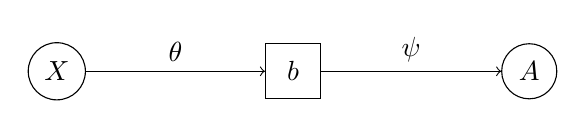
\begin{tikzpicture}[
		roundnode/.style={circle, draw=black, minimum size=7mm},
		squarednode/.style={rectangle, draw=black, minimum size=7mm}
		]
		% nodes
		\node[roundnode] (X) at (0, 0) {$X$};
		\node[squarednode] (b) at (3, 0) {$b$};
		\node[roundnode] (A) at (6, 0) {$A$};
		
		% arrows
		\draw[->] (X.east) -- node[above] {$\theta$} (b.west);
		\draw[->] (b.east) -- node[above] {$\psi$}(A.west);
	\end{tikzpicture}
	\caption{The feature-first block model (FFBM)}
	\label{fig:ffbm}
\end{figure}

Once the block memberships $b$ have been generated, we then draw the graph $A$ from the microcanonical DC-SBM (equation \ref{eqn:A-generation}) with additional parameters encapsulated by $\psi = \{\psi_e, \psi_k\}$.
%
\begin{equation}
	A \sim \textrm{DC-SBM}_{\textrm{MC}} (b, \psi_e, \psi_k)
	\label{eqn:A-generation}
\end{equation}


\subsection{Prior selection}

Before performing any inference, we must specify priors on $\theta$ and $\psi$. For $\theta$ it seems sensible to choose a Gaussian prior, with zero mean and variance matrix $\sigma^2_\theta I$ such that each element of $\theta$ is independent and distributed like $\sim \Gaussian(0, \sigma_\theta^2)$. In vector form, the prior for $\theta$ is therefore:
%
\begin{equation}
	p(\theta) = \Gaussian \left( \theta ; 0, \sigma_\theta^2 I \right)
	\label{eqn:theta-prior}
\end{equation}
%
In our model, the block memberships vector $b$ is an intermediate latent variable and so we are not free to choose a prior for it. Nevertheless, as far as inference on the right-hand-side of figure \ref{fig:ffbm}, we regard $p(b | X)$ as a pseudo-prior on $b$. We can show (appendix \ref{appdx:b|x}) that our choice of prior for $p(\theta)$ in equation \ref{eqn:theta-prior} leads to a uniform $p(b | X)$ in equation \ref{eqn:b-pseudo-prior}.
%
\begin{equation}
	p(b | X) = \int p(b | X, \theta) p(\theta) d\theta = B^{-N}
	\label{eqn:b-pseudo-prior}
\end{equation}
%
This is an enormously important simplification as evaluating $p(b | X)$ does not require an expensive Monte-Carlo integration over the $\theta$-domain nor does it require the exact value of $X$. \citet{Peixoto-Bayesian-Microcanonical} proposes careful choices for the additional microcanonical SBM parameters $\psi$ which we adopt. Peixoto's idea is to write the joint prior on $(b, e, k)$ as a product of conditionals $p(b, e, k) = p(b) p(e | b) p(k | e, b)= p(b) p(\psi | b)$. For our purposes we must insert a conditioning on $X$, to form our pseudo-prior for $b$ and $\psi$, to give equation \ref{eqn:joint-pseudo-prior}.
%
\begin{equation}
	p(b, \psi | X) = p(b | X) p(\psi | b, X) = p(b | X) p(\psi | b)
	\label{eqn:joint-pseudo-prior}
\end{equation}
%
Where we leverage the fact $(\psi \indep X) | b$. We then borrow the priors proposed by \citet{Peixoto-Bayesian-Microcanonical} for $p(\psi | b)$ to complete our model. Please refer to appendix \ref{appdx:sbm} for the exact form of $p(\psi | b)$. All that concerns the main argument is we have a computable form.

	%\subsection{Prior selection}

To complete the description of our Bayesian framework,
priors on $\theta$ and $\psi$ must also be specified. 
We place a Gaussian prior on $\theta$ such that
each element of $\theta$ has an independent ${\cal N}(0,\sigma_\theta^2)$
prior, with hyperparameter $\sigma_\theta^2$:
%
\begin{equation}
	p(\theta) \sim \mathcal{N} \left( \theta ; 0, \sigma_\theta^2 I \right).
	\label{eqn:theta-prior}
\end{equation}
%
This choice of prior gives a very
simple form for the conditional distribution of the block membership vector $b$ given $X$; it is a uniform distribution:
%
\begin{equation}
	p(b | X) = \int p(b | X, \theta) p(\theta) d\theta = B^{-N}.
	\label{eqn:b-pseudo-prior}
\end{equation}
%
The proof is given in Appendix~\ref{appdx:b|x}. This is an important simplification as evaluating $p(b | X)$ does not require an expensive  integration over $\theta$ nor does it depend on $X$.
Peixoto \cite{Peixoto-Bayesian-Microcanonical} proposes careful choices for 
the priors on the additional microcanonical SBM parameters $\psi$, which we adopt without repeating their exact form here. 
The idea is to write the joint distribution on $(b, e, k)$ as a product of 
conditionals, $p(b, e, k) = p(b) p(e | b) p(k | e, b)= p(b) p(\psi | b)$. 
In our case, conditioning on $X$ is also necessary, leading to,
$
p(b, \psi | X) = p(b | X) p(\psi | b, X) = p(b | X) p(\psi | b),
$
where we used the fact $\psi$ and $X$ are conditionally 
independent given $b$.
All that concerns the main argument is that $p(\psi|b)$ has
an easily computable form.
	
	\section{Inference}
\label{sec:inference}

Now that we have defined the FFBM, we wish to leverage it to perform inference. Suppose we are presented with a vertex-labelled graph $(A, X)$; the goal is to draw samples for $\theta$ according to the posterior given the observed data:
%
\begin{equation}
	\label{eqn:theta-target}
	\theta^{(t)} \sim p(\theta | A, X)
\end{equation}
%
However, generating these samples is not easily done in practice. We therefore propose an iterative approach. We first draw samples $b^{(t)}$ from the block membership posterior (equation \ref{eqn:b-samples}) and then use each $b^{(t)}$ to draw samples for $\theta$ as in equation \ref{eqn:theta-samples}. 
%
\begin{align}
	b^{(t)} &\sim p \Big( b | A, X \Big)  \label{eqn:b-samples}\\
	\theta^{(t)} &\sim p\Big(\theta | X, b^{(t)} \Big) \label{eqn:theta-samples}
\end{align}
%
Both of these sampling steps can be implemented with a Markov Chain through the Metropolis-Hastings algorithm \cite{hastings-alg}. We just need to define a proposal distribution $q(x, x')$ for proposing a move $x \rightarrow x'$ and be able to evaluate an un-normalised form of the target distribution, denoted $\pi(\cdot)$, point-wise. The proposed move is then accepted with probability $\alpha$ (equation \ref{eqn:mh-accept}) else it is rejected and we stay at $x$.
%
\begin{equation}
	\alpha(x, x') = \min \left( \frac{\pi(x') q(x', x)}{\pi(x) q(x, x')} , 1 \right)
	\label{eqn:mh-accept}
\end{equation}
%
This accept-reject step ensures the resulting Markov Chain is in detailed balance with the target distribution $\pi(\cdot)$. What we propose in equations \ref{eqn:b-samples} and \ref{eqn:theta-samples} is therefore implemented through a 2-level Markov chain. The resulting samples for $\theta^{(t)}$ are unbiased in the sense that the expectation of their distribution is the posterior we are targetting:
%
\begin{equation}
\Expect_{b^{(t)}} \left[p \left( \theta | X, b^{(t)} \right) \right] = \sum_{b \in [B]^N} p(\theta | X, b) p(b | A, X) = \sum_{b \in [B]^N} p(\theta, b | A, X) = p(\theta | A, X)
\label{eqn:theta-unbiased}
\end{equation}
%
This is an example of a pseudo-marginal approach. Indeed, \citet{pseudo-marginal} show that the unbiased result in equation \ref{eqn:theta-unbiased} is sufficient to prove that for large enough $t$, $\theta^{(t)} \sim \Expect_{b^{(i)}} \left[ p(\theta | X, b^{(t)})\right] = p(\theta 
| A, X)$ which is exactly the distribution we are targetting (equation \ref{eqn:theta-target}).
%
\begin{figure}[!h]
	\centering

	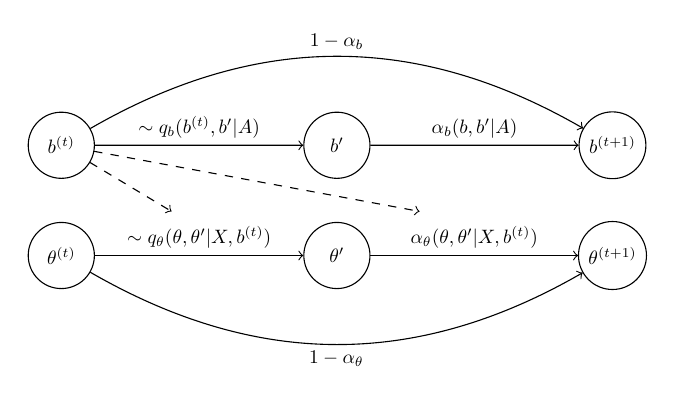
\begin{tikzpicture}[
		scale=0.7, every node/.style={transform shape},
		roundnode/.style={circle, draw=black, minimum size=12mm},
		squarednode/.style={rectangle, draw=black, minimum size=12mm}
		]
		% nodes
		\node[roundnode] (b0) at (0, 2) {$b^{(t)}$};
		\node[roundnode] (b1) at (5, 2) {$b'$};
		\node[roundnode] (b2) at (10, 2) {$b^{(t+1)}$};
		\node[roundnode] (t0) at (0, 0) {$\theta^{(t)}$};
		\node[roundnode] (t1) at (5, 0) {$\theta'$};
		\node[roundnode] (t2) at (10, 0) {$\theta^{(t+1)}$};
		
		% arrows
		\draw[->] (b0) to node[above] {$\sim q_b(b^{(t)}, b' | A)$} (b1);
		\draw[->] (b1) to node[above] {$\alpha_b (b, b' | A)$} (b2);
		\draw[->] (b0) [out=30, in=150] to node[above] {$1-\alpha_b$} (b2);
		
		\draw[->] (t0) to node[above] {$\sim q_\theta(\theta, \theta' | X, b^{(t)})$} (t1);
		\draw[->] (t1) to node[above] {$\alpha_\theta (\theta, \theta' | X, b^{(t)})$} (t2);
		\draw[->] (t0) [out=-30, in=-150] to node[below] {$1-\alpha_\theta$} (t2);
		
		\draw[dashed, ->] (b0) to (2, 0.8);
		\draw[dashed, ->] (b0) to (6.5, 0.8);
		
	\end{tikzpicture}
	\caption{Sampling sequence}
	\label{fig:samp-sequence}
\end{figure}

The reason we split the Markov chain into two stages is because the summation over all latent states $b \in [B]^N$ required to directly compute the likelihood $p(A| X, \theta) = \sum_{b \in [B]^N} p(A | b) P(b | X, \theta)$ is intractable -- $O(B^N)$. Figure \ref{fig:samp-sequence} shows an overview of the proposed method. We have introduced subscripts and conditionings to make explicit what variables each step utilises. We note the power of the simplification given by equation \ref{eqn:b-pseudo-prior}. As $p(b| X)$ does not depend on the exact value of X, we do not need to know the value of $X$ to perform the sampling on $b$. Conversely, for the $\theta^{(t)}$ samples, we use only $b^{(t)}$ but not $A$ as $(\theta \indep A) | b$.

\FloatBarrier

\subsection{Sampling block memberships}

\citet{Peixoto-MCMC} proposes a Monte Carlo method which we will base our approach on. It relies on writing the posterior in the following form:
%
\begin{equation}
	p(b | A, X) \propto p(A | b, X) \cdot p(b | X) = \pi_b(b)
\end{equation}
%
Now $\pi_b(\cdot)$ is the un-normalised density we wish to sample from for the $b$-chain. In other words, we wish to construct a Markov chain that has $\pi_b(\cdot)$ as its invariant distribution. We can break $\pi_b$ down as follows:
%
\begin{equation}
	\pi_b(b) = p(b|X) \sum_{\psi} \nolimits p(A , \psi | b, X) \\
	= p(b|X) p(A, \psi^* | b, X) \\
	= p(A | b, \psi^*) \cdot p(\psi^* | b) \cdot p(b | X)
\end{equation}
%
Since we are using the microcanonical SBM formulation, there is only one value of $\psi$ that is compatible with the given $(A, b)$ pair (given in equation \ref{eqn:sbm-constraints}). We denote this value $\psi^* = \{\psi_k^*, \psi_e^*\}$. Therefore, the summation over all $\psi$ reduces to just the single $\psi^*$ term; this is the power of the microcanonical formulation. We also define the microcanonical entropy of the configuration as.
%
\begin{equation}
	S(b) = - \log \pi_b(b) = - \Big( \log p(A | b, \psi^*) + \log p(\psi^*, b | X) \Big)
	\label{eqn:dl-form}
\end{equation}
%
This entropy can equally be thought of as the description length of the graph. The exact form of the proposal $q_b$ is explored thoroughly by \citet{Peixoto-MCMC} and not repeated here. There is a widely used library for Python made available under LGPL called \verb*|graph-tool| \cite{peixoto_graph-tool_2014}, which implements this algorithm. The only modification we make is in the block membership prior $p(b)$ which we replace with $p(b|X)=B^{-N}$, which cancels out in the MH accept-reject step as it is independent of $b$.

\subsection{Sampling feature-to-block generator parameters}

The invariant distribution we wish to target for the $\theta$ samples is the posterior of $\theta$ given the values of the pair $(X, b)$. We write this as follows:
%
\begin{equation}
	\pi_\theta(\theta) \propto p(\theta | X, b) \propto p(b | X, \theta) p(\theta) \propto \pi_\theta (\theta) \propto  \exp \left( - U(\theta) \right)
\end{equation}
%
Where we have introduced $U(\theta)$ equal to the negative log posterior. We define $y_{ij} \coloneqq \one \left\{ b_i = j \right\}$ and $a_{ij} \coloneqq \phi_j(x_i; \theta)$. Discarding constant terms, we can write $U(\theta)$ as in equation \ref{eqn:U-form} (refer to appendix \ref{appdx:form-U} for the derivation).
%
\begin{equation}
	U(\theta) = \left( \sum_{i=1}^{N} \sum_{j=1}^{B} y_{ij} \log \frac{1}{a_{ij}} \right)
	+ \frac{1}{2\sigma_\theta^2} ||\theta||^2 = N \cdot \Lcal(\theta) + \frac{1}{2\sigma_\theta^2} ||\theta||^2
	\label{eqn:U-form}
\end{equation}
%
$U(\theta)$ in equation \ref{eqn:U-form} appears a typical objective function for neural network training. The first term is introduced by the likelihood. We collect it into $N \cdot \Lcal(\theta)$, which is the cross-entropy between the graph-predicted and feature-predicted block memberships summed over all vertices. The second term of equation \ref{eqn:U-form} -- introduced by the prior -- brings a form of regularisation, guarding against over-fitting. Different to traditional applications, our goal is not to find the minimiser of $U(\theta)$ but to draw samples from the posterior $\pi_\theta(\cdot) \propto \exp(-U(\cdot))$. We can use $\nabla U$ as a useful heuristic to bias our proposal towards regions of higher target density. We therefore adopt the Metropolis-adjusted Langevin algorithm (MALA) -- first proposed by \citet{mala-tweedie}. Given the current sample $\theta$, we generate a new sample $\theta'$ according to equation \ref{eqn:theta-update}.
%
\begin{align}
	\theta' &= \theta - h \nabla U(\theta) + \sqrt{2h} \cdot \xi
	\label{eqn:theta-update} \\
	\therefore q_\theta(\theta, \theta') &= \Gaussian \left( \theta' ; \theta - h \nabla U(\theta), 2h I \right)
	\label{eqn:theta-proposal}
\end{align}
%
Where $\xi \sim \Gaussian(0, I)$ and $h$ is a step-size parameter -- which may vary with the sample index (appendix \ref{appdx:step-size} explores this more fully). Without the injected noise term, MALA is equivalent to gradient descent. We require the noise term $\xi$ to fully explore the parameter space. We can write the proposal distribution $q_\theta$ as in equation \ref{eqn:theta-proposal}. The term $\nabla U$ has an easy to compute analytic form (derived in Appendix \ref{appdx:gradu}). By noting that $\theta = \{w_k\}_{k=1}^{B}$, we write the derivative with respect to each $w_k$ as:
%
\begin{equation}
	\frac{\partial U}{\partial w_k} = - \left( \sum_{i=1}^{N} \Big\{ \tilde{x}_i (y_{ik} - a_{ik}) \Big\} - \frac{w_k}{\sigma_\theta^2} \right)
	\label{eqn:U-derivative}
\end{equation}
%
After a proposed move is generated, in typical Metropolis-Hastings fashion we accept the move with probability $\alpha_\theta$, as in equation \ref{eqn:mh-accept}.

\subsection{Sampling sequence}

Up to this point, each $\theta^{(t)}$ update uses its corresponding $b^{(t)}$ sample. This means that the evaluation of $U(\theta)$ and $\nabla U(\theta)$ has high variance. This may lead to longer burn-in for the resulting Markov chain. The only link between $b^{(t)}$ and $\theta^{(t)}$ is in the evaluation of $U(\theta)$ and $\nabla U(\theta)$ which depends only on the matrix $y^{(t)}$ with entries $y_{ij}^{(t)} \coloneqq \one\{b_i^{(t)} = j\}$. We would rather deal with the expectation of each $y_{ij}^{(t)}$:
%
\begin{equation}
	\Expect \left[ y_{ij}^{(t)} \right] = \Expect_{b^{(t)}} \left[ \one(b_{i}^{(t)} = j) \right]
	= p(b_i = j | A, X)
\end{equation}
%
We can obtain an unbiased estimate for this quantity using the set of $b$-samples. However, as with all MCMC methods, we must only uses samples after burn-in and thinning have been applied. We introduce $\Tcal_b$ to denote the retained set of indices for the $b$-samples and $\Tcal_\theta$ similarly for the $\theta$-chain. An in-depth discussion of how these sets are chosen is given in appendix \ref{appdx:burn-in-thinning}. The unbiased estimate for $y_{ij}^{(t)}$ using the restricted sample set $\Tcal_b$ is denoted $\hat{y}_{ij}$ and has form:
%
\begin{equation}
	\hat{y}_{ij} \coloneqq \frac{1}{|\Tcal_b|} \sum_{t \in \Tcal_b} y_{ij}^{(t)} = \frac{1}{|\Tcal_b|} \sum_{t \in \Tcal_b} \one\{b_i^{(t)} = j\}
\end{equation}
%
We choose to feed each $\theta^{(t)}$ update step the same matrix $\hat{y}$ for all $t$ rather than the corresponding $y^{(t)}$. This means we no longer need to run the $b$ and $\theta$ Markov chains concurrently. Instead, we run the $b$-chain to completion and use it to generate $\hat{y}$. This affords us the flexibility to vary the lengths of the $b$ and $\theta$-chains. Furthermore, the changeover from $y^{(t)}$ to $\hat{y}$ reduces the burn-in time for the $\theta$-chain by reducing the variance in our evaluation of $U$ and $\nabla U$. A description of the overall algorithms is given in appendix \ref{appdx:algorithms}.

\subsection{Dimensionality reduction}
\label{sec:dim-reduction}

Once we have the samples $\left\{ \theta^{(t)} \right\} \sim p(\theta | A, X)$, we can compute the empirical mean and standard deviation of each component of $\theta$. Switching back to matrix notation we define $\theta = W$, such that $W_{ij}$ is the weight component for block $i$ and feature $j$, we can define:
%
\begin{equation}
	\hat{\mu}_{ij} \coloneqq \frac{1}{|\Tcal_\theta|} \sum_{t \in \Tcal_\theta} W_{ij}^{(t)} \qquad \textrm{and} \qquad
	\hat{\sigma}_{ij} \coloneqq \frac{1}{|\Tcal_\theta|} \sum_{t \in \Tcal_\theta} \left( W_{ij}^{(t)} - \hat{\mu}_{ij} \right)^2
\end{equation}
%
A simple heuristic to discard the least important features requires specifying a cutoff $c > 0$ and a multiplier $k > 0$. We define the function $\Fcal_i(j)$ as in \ref{eqn:fij} then only keep features with indices $d \in \Dcal'$, where $\Dcal'$ is constructed as in equation \ref{eqn:kept-feature-set}.
%
\begin{align}
	\Fcal_i(j) &\coloneqq (\hat{\mu}_{ij} - k \hat{\sigma}_{ij}, \hat{\mu}_{ij} + k \hat{\sigma}_{ij}) \cap (-c, +c)
	\label{eqn:fij} \\
	\Dcal' &\coloneqq \left\{ j \in [D] : \exists i \in [B] \textrm{ s.t. }  \Fcal_i(j) \neq \emptyset \right\}
	\label{eqn:kept-feature-set}
\end{align}
%
Intuitively, this means discarding any feature for which $\hat{\mu}_{ij} \pm k\hat{\sigma}_{ij}$ lies within or spans the null region $(-c, c)$ for all block indices. If we were to use the Laplace approximation for the posterior $p(W_{ij} | A, X) \approx \Gaussian(W_{ij}; \mu_{ij}, \sigma_{ij})$, then this is effectively a hypothesis test on the value of $W_{ij}$ (equation \ref{eqn:hyp-test-discard}). $\Dcal'$ then comprises all features $i$ for which $H_1$ is accepted at least once for some $j \in [B]$.
%
\begin{equation}
	H_0: |\mu_{ij}| \leq c \qquad
	H_1: |\mu_{ij}| > c
	\label{eqn:hyp-test-discard}
\end{equation}
%
The multiplier $k$ determines the degree of significance of the result. However, as the Laplace approximation is not exact we will only treat this dimensionality reduction method as a useful heuristic and not an exact method. Conversely, we could fix $k=k_0$ and the dimension of our reduced feature set $|\Dcal'|=D'$. We would then like to find the largest value of $c$ such that $|\Dcal'|=D'$ given $k=k_0$. This is summarised in equation \ref{eqn:c-star}. This approach is often preferred as it fixes the number of reduced dimensions.
%
\begin{equation}
	c^* = \argmax_{c>0} (c : |\Dcal'| = D', k=k_0)
	\label{eqn:c-star}
\end{equation}
	%\subsection{Sampling block memberships}

To generate the required $b$-samples, we adopt the MCMC
procedure of
\cite{Peixoto-MCMC},
which relies on writing the posterior in the following form,
%
\begin{equation}
	p(b | A, X) \propto p(A | b, X) \cdot p(b | X) = \pi_b(b),
\end{equation}
%
where $\pi_b(\cdot)$ denotes the un-normalised target density.
Since we are using the microcanonical SBM formulation, there is only one 
value of $\psi$ that is compatible with the given $(A, b)$ pair;
recall the constraints in~(\ref{eqn:sbm-constraints}).
We denote this value $\psi^* = \{\psi_k^*, \psi_e^*\}$. Therefore, 
the summation over all $\psi$ needed to evaluate $p(A | b, X)$ reduces to just the single $\psi^*$ term:
$p(A | b, X) = \sum_{\psi} \nolimits p(A , \psi | b, X) = p(A, \psi^* | b, X)$.
In
this context, the microcanonical entropy of the configuration $b$
is,
%
\begin{equation}
	S(b) \triangleq - \log \pi_b(b) = - \Big( \log p(A | b, \psi^*) + \log p(\psi^*, b | X) \Big),
	\label{eqn:dl-form}
\end{equation}
%
which can be thought of as the optimal
``description length'' of the graph. 
This expression will later be employed 
to help evaluate experimental results. 
The exact form of the proposal $q_b$ is explored thoroughly in
\cite{Peixoto-MCMC} and not repeated here. We use the \verb*|graph-tool| \cite{peixoto_graph-tool_2014}
library for Python, which implements this algorithm.
The only modification is in 
the prior $p(b)$ that we replace with $p(b|X)=B^{-N}$, 
which cancels out in the MH accept-reject step as it is independent of $b$.

\subsection{Sampling feature-to-block generator parameters}
\label{s:sfb}

The target distribution for the required $\theta$-samples 
is the posterior of $\theta$ given the values of the pair $(X, b)$. 
We write this as,
%
\begin{equation}
	\pi_\theta(\theta) \propto p(\theta | X, b) \propto p(b | X, \theta) p(\theta) \propto  \exp \left( - U(\theta) \right),
	\label{eq:U}
\end{equation}
%
where $U(\theta)$ denotes the negative log-posterior. Let $y_{ij} \triangleq \boldsymbol{1} \left\{ b_i = j \right\}$ and $a_{ij} \triangleq \phi_j(x_i; \theta)$. 
Discarding constant terms, $U(\theta)$ can be expressed as,
%
\begin{equation}
	U(\theta) = \left( \sum_{i \in [N]} \sum_{j \in [B]} y_{ij} \log \frac{1}{a_{ij}} \right)
	+ \frac{1}{2\sigma_\theta^2} \|\theta\|^2 = N \cdot \mathcal{L}(\theta) + \frac{1}{2\sigma_\theta^2} \|\theta\|^2;
	\label{eqn:U-form}
\end{equation}
%
see Appendix \ref{appdx:form-U}. The function $U(\theta)$ is a typical objective function for neural network training. The first term $N \cdot \mathcal{L}(\theta)$ is introduced by the likelihood and represents the cross-entropy between the graph-predicted and feature-predicted block memberships. 
The second term, introduced by the prior, brings a form of regularisation, guarding against over-fitting. In order to draw samples from the posterior 
$\pi_\theta \propto \exp(-U)$ we adopt the Metropolis-adjusted Langevin 
algorithm (MALA) \cite{mala-tweedie}, which uses $\nabla U$ to bias the 
proposal towards regions of higher density. Given the current 
sample $\theta$, a proposed 
new sample $\theta'$ is generated from,
%
\begin{equation*}
	\theta' \sim q_\theta\big(\theta, \theta'\big) 
	= \mathcal{N} \big( \theta' ; \theta - h \nabla U(\theta), 2h I \big),
\end{equation*}
%
where $\xi \sim \mathcal{N}(0, I)$ and $h$ is a step-size parameter 
which may vary with the sample index.
Without the injected noise term $\xi$, MALA is equivalent to gradient descent. We require $\xi$ to fully explore the parameter space. 
The term $\nabla U$ has an easy to compute analytic form (derived in Appendix \ref{appdx:form-U}).

\subsection{Sampling sequence}
\label{s:ss}

So far, each $\theta^{(t)}$ update has used its corresponding $b^{(t)}$ sample. This means the evaluation of $U^{(t)}$ and $\nabla U^{(t)}$ has high variance, leading to longer burn-in and possibly slower MCMC convergence. The only link between $b^{(t)}$ and $\theta^{(t)}$ is in the evaluation of $U^{(t)}$ and $\nabla U^{(t)}$ which depends only on the matrix $y^{(t)}$ with entries $y_{ij}^{(t)} \triangleq \boldsymbol{1}\{b_i^{(t)} = j\}$. We would rather deal with the expectation of each $y_{ij}^{(t)}$:
%
\begin{equation}
	\mathbb{E} \left[ y_{ij}^{(t)} \right] = \mathbb{E}_{b^{(t)}} \left[ \boldsymbol{1} \left( b_{i}^{(t)} = j \right) \right]
	= p(b_i = j | A, X).
\end{equation}
%
An unbiased estimate for this can be obtained using 
the thinned $b$-samples after burn-in.
Let $\mathcal{T}_b$  denote the retained set of indices 
for the $b$-samples and $\mathcal{T}_\theta$ similarly for the $\theta$-chain. 
The unbiased estimate for $y_{ij}^{(t)}$ is then:
%
\begin{equation}
	\hat{y}_{ij} \triangleq \frac{1}{|\mathcal{T}_b|} \sum_{t \in \mathcal{T}_b} y_{ij}^{(t)} = \frac{1}{|\mathcal{T}_b|} \sum_{t \in \mathcal{T}_b} \boldsymbol{1}\{b_i^{(t)} = j\}.
	\label{eqn:y-hat}
\end{equation}
%
The same matrix $\hat{y}$ is used in each $\theta^{(t)}$ update step.
This way, it is not necessary to run the $b$ and $\theta$ Markov chains 
concurrently. Instead, we run the $b$-chain to completion and use it 
to generate $\hat{y}$ also allowing us to vary the lengths of each.

\subsection{Dimensionality reduction}
\label{sec:dim-reduction}

The complexity of evaluating $U$ and $\nabla U$ is linear in 
the dimension of the feature space $D$,
so there is computational incentive to reduce $D$.
Given the samples $\left\{ \theta^{(t)} \right\}$, we can compute the empirical mean and standard deviation of each component of $\theta$. 
Switching to the matrix notation $W$ for $\theta$,
let:
%
\begin{equation}
	\hat{\mu}_{ij} \triangleq \frac{1}{|\mathcal{T}_\theta|} \sum_{t \in \mathcal{T}_\theta} W_{ij}^{(t)} \qquad \textrm{and} \qquad
	\hat{\sigma}_{ij}^2 \triangleq \frac{1}{|\mathcal{T}_\theta|} \sum_{t \in \mathcal{T}_\theta} \left( W_{ij}^{(t)} - \hat{\mu}_{ij} \right)^2.
\end{equation}
%
A simple heuristic to discard the least important features requires specifying a cutoff $c > 0$ and a multiplier $k > 0$. We define the function $\mathcal{F}_i(j)$ 
as in~(\ref{eqn:fij}) and only keep features with indices $d \in \mathcal{D}'$, where $\mathcal{D}'$ is given in~(\ref{eqn:kept-feature-set}).
%
\begin{align}
	\mathcal{F}_i(j) &\triangleq (\hat{\mu}_{ij} - k \hat{\sigma}_{ij}, \hat{\mu}_{ij} + k \hat{\sigma}_{ij}) \cap (-c, +c),
	\label{eqn:fij} \\
	\mathcal{D}' &\triangleq \left\{ j \in [D] : \exists i \in [B] \textrm{ s.t. }  \mathcal{F}_i(j) = \emptyset \right\}.
	\label{eqn:kept-feature-set}
\end{align}
%
Intuitively, this means discarding any feature $j$ for which 
$(\hat{\mu}_{ij} - k\hat{\sigma}_{ij}, \hat{\mu}_{ij} + k \hat{\sigma}_{ij})$ overlaps with
$(-c, c)$ for all $i$. If we were to use the Laplace approximation for the posterior $p(W_{ij} | A, X) \approx \mathcal{N}(W_{ij}; \hat{\mu}_{ij}, \hat{\sigma}_{ij}^2)$, then this would be analogous to a hypothesis test on the magnitude of $W_{ij}$ compared to $c$ with multiplier $k$ in~(\ref{eqn:fij}) determining the degree of significance of the result. Conversely, if we want to fix the number of dimensions in our reduced feature set $|\mathcal{D}'|=D'$, the problem then becomes finding the largest value of $c$ such that $|\mathcal{D}'|=D'$ given $k=k_0$:
%
\begin{equation}
	c^* = {\operatorname{argmax}} \{c>0\; : \;|\mathcal{D}'| = D', k=k_0\}.
	\label{eqn:c-star}
\end{equation}


	
	\section{Experiments}
\label{sec:experiments}

We apply the outlined methods to a variety of datasets:

\begin{itemize}
	\item \textbf{Political books} \cite{polbooks} ($N=105, E=441, D=3$) -- network of Amazon political book sales, published close to the 2004 presidential election. Two books are connected if they were frequently co-purchased. Vertex features encode the political affiliation of the author (liberal, conservative, or neutral).
	\item \textbf{Primary school dynamic contacts} \cite{schools} ($N=238, E=5539, D=13$) -- network of face-to-face contacts amongst students and teachers at a primary school in Lyon, France. Vertex features include class membership (one of 10 values: 1A-5B), gender (male, female) and teacher status encoded as an 11th school-class. We choose to analyse just the second day of results.
	\item \textbf{Facebook egonet} \cite{fb-snap} ($N=747, E=30025, D=480$) -- an assortment of Facebook users' friends lists. Vertex features are fully anonymised and encode information about each user's education history, languages spoken, gender, home-town, birthday etc. We focus on the egonet with id 1912.
\end{itemize}
%
We first require metrics to assess model performance. We define the average
description length per entity (nodes and edges) $\bar{S}_e$ as a suitable metric to gauge the SBM fit:
%
\begin{equation}
	\bar{S}_e \coloneqq \frac{1}{(N+E) |\Tcal_b|} \sum_{t\in \Tcal_b} S \left( b^{(t)} \right).
	\label{eqn:mean-dl}
\end{equation}

Next, to assess the performance of the feature-to-block predictor, 
we randomly partition the vertex set $[N]$ into training and test sets: $\Gcal_0$ and $\Gcal_1$.
The $b$-chain is run using the whole network but we only use vertices $v \in \Gcal_0$ to train the $\theta$-chain. As $|\Gcal_0| \neq |\Gcal_1|$ in general, we use the average cross-entropy loss 
over each set to gauge fit,
%
\begin{equation}
	\bar{\Lcal}_\star \coloneqq \frac{1}{|\Tcal_\theta|} \sum_{t \in \Tcal_\theta} \Lcal_\star^{(t)},
	\quad \textrm{where} \quad
	\Lcal_\star^{(t)} \coloneqq \frac{1}{|\Gcal_\star|} \sum_{i \in \Gcal_\star}\sum_{j \in [B]} \hat{y}_{ij} \log \frac{1}{\phi_j \left(x_i; \theta^{(t)} \right)},
	\label{eqn:cross-entropy-loss}
\end{equation}
%
where $\star \in \{0, 1\}$ toggles between the training and test sets.
%
Nevertheless, the cross-entropy loss is a coarse measure of fit. We wish to define a new measure of fit specific to each detected block. Let us define
$
	\Bcal_\star(j) \coloneqq \{i \in \Gcal_\star : \hat{b}_i = j\}
$
where
$ 
	\hat{b}_i \coloneqq \argmax_j \hat{y}_{ij}.
$
Now $\Bcal_\star(j)$ is the set of vertices that have maximum a posteriori probability of belonging to block $j$. We now define the accuracy for block $j$ as,
%
\begin{equation}
	\eta_\star(j) \coloneqq \frac{1}{|\Bcal_\star (j)| \cdot 
	|\Tcal_\theta| } 
	\sum_{i \in \Bcal_\star (j)}  \sum_{t \in \Tcal_\theta}
	\one \left\{\hat{b}_i = \argmax_j \phi_j \left( x_i; \theta^{(t)} \right) \right\}.
	\label{eqn:accuracy}
\end{equation}

This effectively tests whether the feature-to-block and the graph-to-block predictions agree in their largest component. We call this metric, $\eta_\star(j)$, the {\em block-accuracy} for block $j$. It is clearly bounded $0 \leq \eta_\star(j) \leq 1$, with an accuracy of 1 meaning perfect agreement for the vertices in detected block $j$.

Table~\ref{tab:results} summarises the results for each experiment. 
We see that the dimensionality reduction procedure 
brings the training and test losses closer together. This implies that 
the features we keep are indeed correlated with the underlying graphical 
partition and that the approach generalises correctly. The test loss variance is higher than the training loss variance as the test set is smaller and so more susceptible to variability in its construction.
%
The average description length per entity,
$\bar{S}_e$, of the graph, 
has very small variance, suggesting that
the detected communities can be found reliably (to within an arbitrary 
relabelling of blocks).

\paragraph{\textbf{Political books.}}

We choose to partition the network into $B=3$ communities as we only have this many distinct values for political affiliation.
From Figure~\ref{fig:polbooks-null} we see that all 3 blocks have a distinct political affiliation as their largest positive component.  
Furthermore, the training and test losses from Table~\ref{tab:results}  
are very similar and both are low in magnitude. This is strong evidence 
that political affiliation is a very appropriate explanatory 
variable for the overall network structure.
%
However, from Figure~\ref{fig:polbooks-accuracy} we see that block 1 has low accuracy. 
This suggests that detected block 1 is not solely composed of ``neutral" books but also 
contains some ``liberal" and ``conservative" authors. Examining 
Figure~\ref{fig:polbooks-graph}, we see the majority of paths between blocks 2 and 3 go through block 1.
Block 1 is in effect a bridge between the ``conservative'' and ``liberal'' blocks so it is unsurprising that some of these leak into block 1.

\paragraph{\textbf{Primary school.}}

We choose the number of communities $B=10$, in line with the total number of 
school classes. Only the pupils' class memberships (1A-5B) survive
the dimensionality-reduction process (Figure~\ref{fig:school-null});
gender and teacher/student status have been discarded,
meaning these are poor predictors of overall macro-structure.
%
The vast majority of blocks are composed of a single class. 
However, some blocks have two comparably strong classes as their predictors (e.g. blocks 2 and 5). 
Conversely, some classes are found to extend over two 
detected blocks (class 2B spans blocks 8 and 9) but we do 
not have a feature which explains the division.
%
Figure~\ref{fig:school-accuracy} shows excellent accuracy for the majority of blocks. In fact the only blocks with low accuracy are those that have a school-class span two blocks such that we cannot reliably distinguish between the two. This is more pronounced when we apply hard classification rather than the soft cross-entropy loss. Perhaps there are unobserved features which explain this divide.

\paragraph{\textbf{Facebook egonet.}}

The retained features 
(Figure~\ref{fig:fb-null}) are those that best explain the high-level 
community structure. The majority of these are education related. 
Nevertheless, for $D'=10$ we only have good explanations for some of the detected blocks; several blocks in 
Figure~\ref{fig:fb-null} do not have high-magnitude components. This is further emphasised by the disparate accuracies in Figure~\ref{fig:fb-accuracy}.
%
For a high-dimensional feature-space, it is likely that a particular
feature may uniquely identify a small set of vertices; if these are all in the same block, then the classifier may overfit despite the penalty imposed by the prior. Indeed, we see in
Figure~\ref{fig:fb-null} that the feature birthday-5 has a very high weight as it relates to block 1 – but it is unlikely that birthdays determine graphical structure.
\begin{table}[!ht]
	\centering
	\caption{Results averaged over $n=10$ iterations (mean $\pm$ std. dev.).}
	\label{tab:results}
	\resizebox{\textwidth}{!}{%
		\begin{tabular}{c|ccc|c|cc|ccc}
			Dataset  & $B$ & $D$ & $D'$ & $\bar{S}_e$ & $\bar{\mathcal{L}}_0$ & $\bar{\mathcal{L}}_1$ & $c^*$ & $\bar{\mathcal{L}}_0'$ & $\bar{\mathcal{L}}_1'$  \\ \hline
			Polbooks & 3 & 3 & -- & $2.250 \pm 0.000$ & $0.563 \pm 0.042$ & $0.595 \pm 0.089$ & -- & -- & -- \\
			School & 10 & 13 & 10 & $1.894 \pm 0.004$ & $0.787 \pm 0.127$ & $0.885 \pm 0.129$ & $1.198 \pm 0.249$ & $0.793 \pm 0.132$ & $0.853 \pm 0.132$ \\
			FB egonet & 10  & 480 & 10 & $1.626 \pm 0.003$ & $1.326 \pm 0.043$ & $1.538 \pm 0.069$ & $0.94 \pm 0.019$ & $1.580 \pm 0.150$ & $1.605 \pm 0.106$
		\end{tabular}
	}
\end{table}

\begin{figure}[!ht]
	\centering
	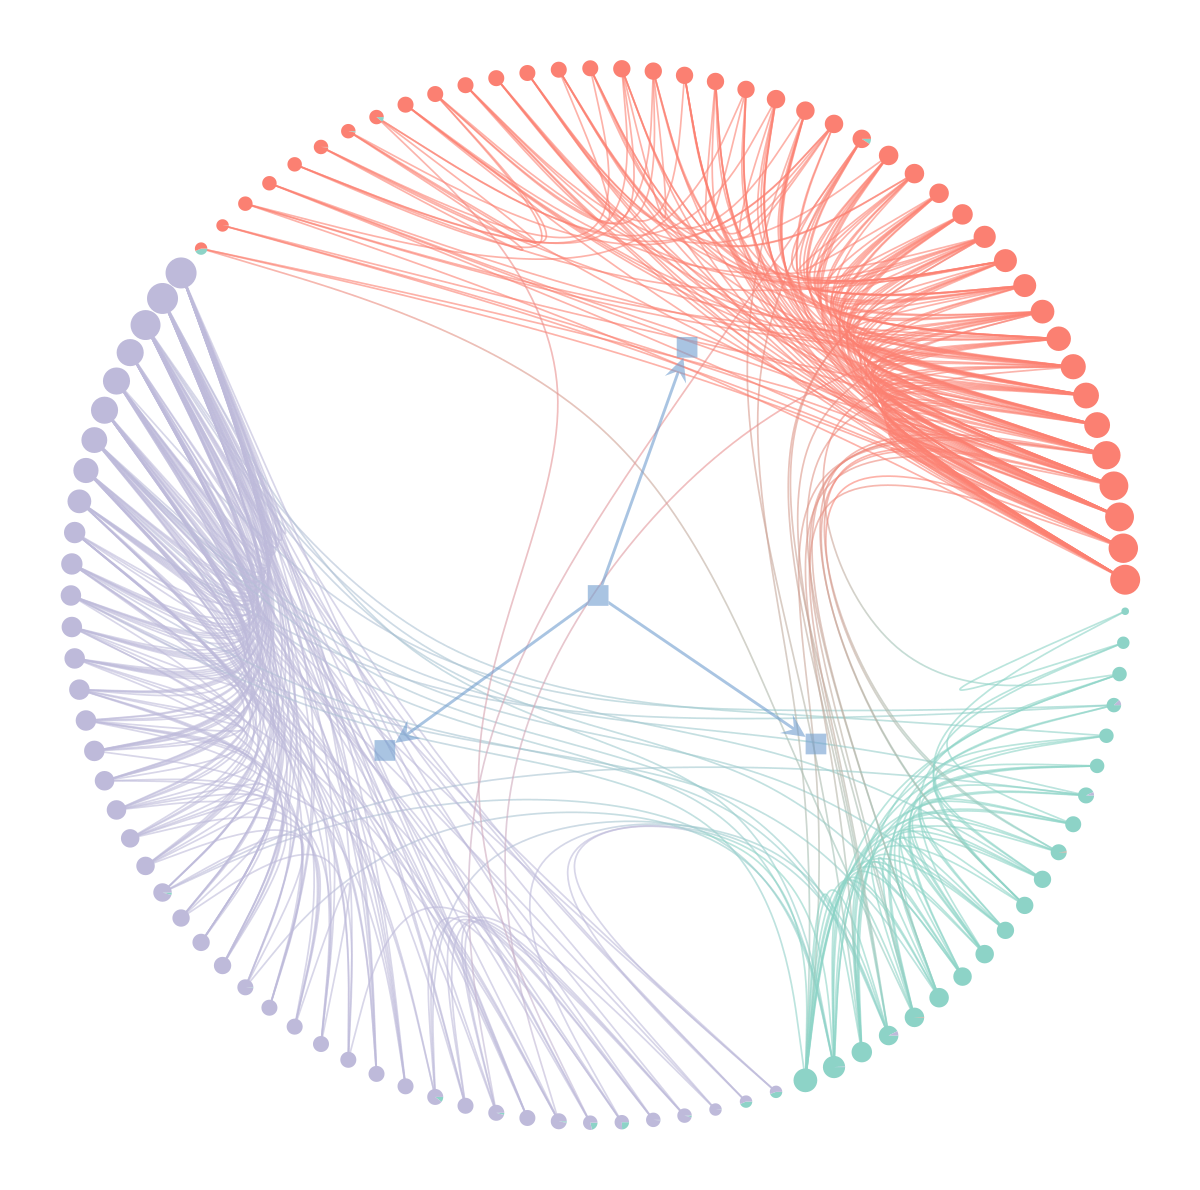
\includegraphics[width=0.28\linewidth]{img/polbooks-graph.png}
	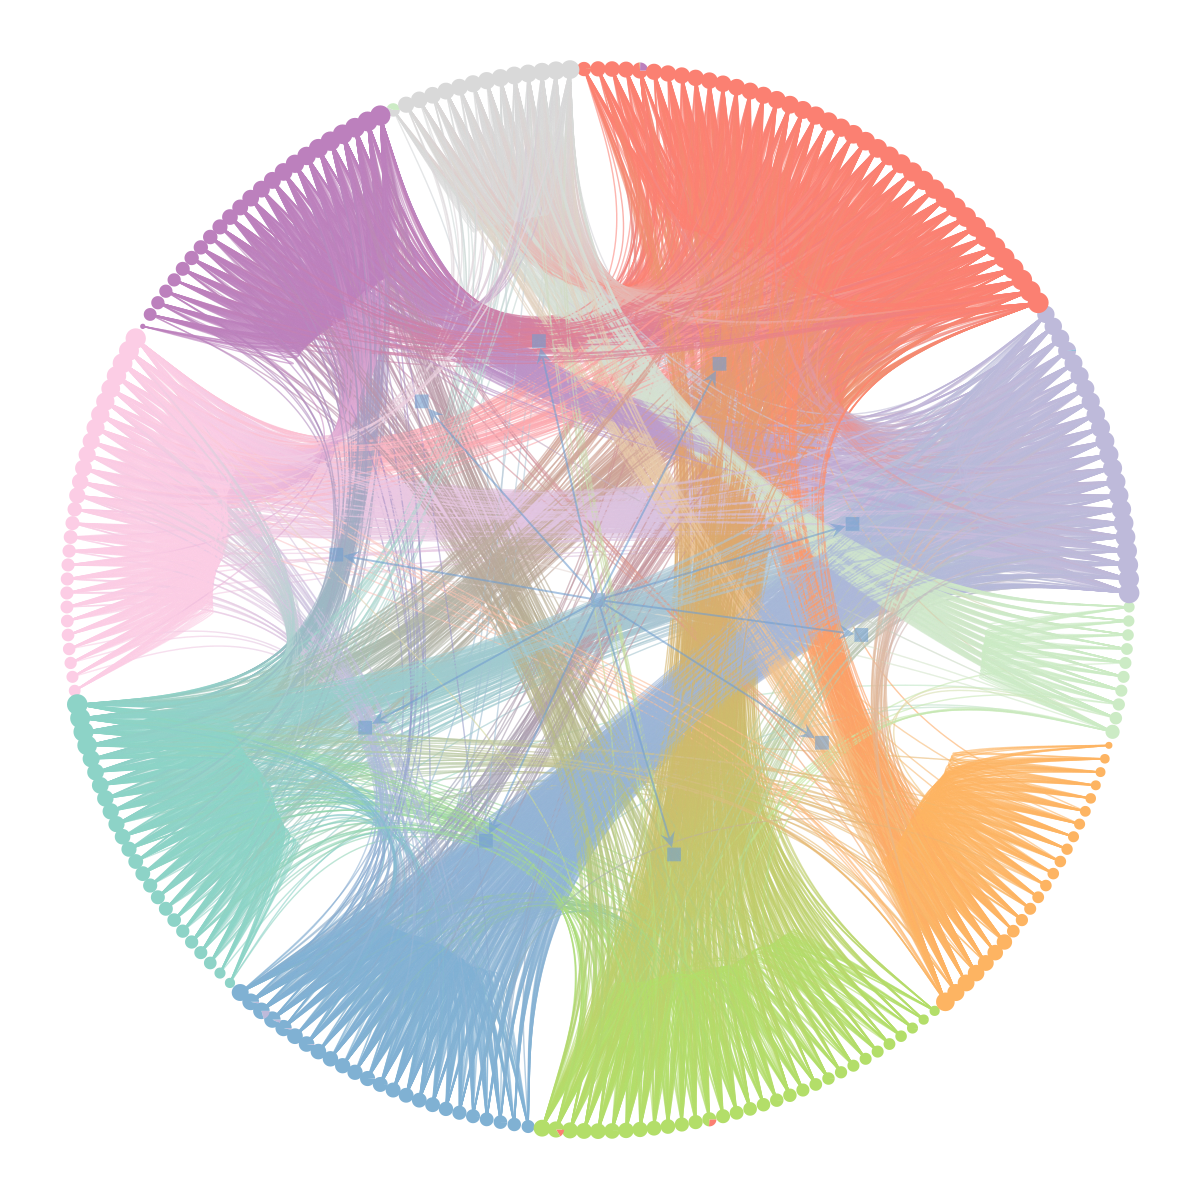
\includegraphics[width=0.28\linewidth]{img/school-graph.png}
	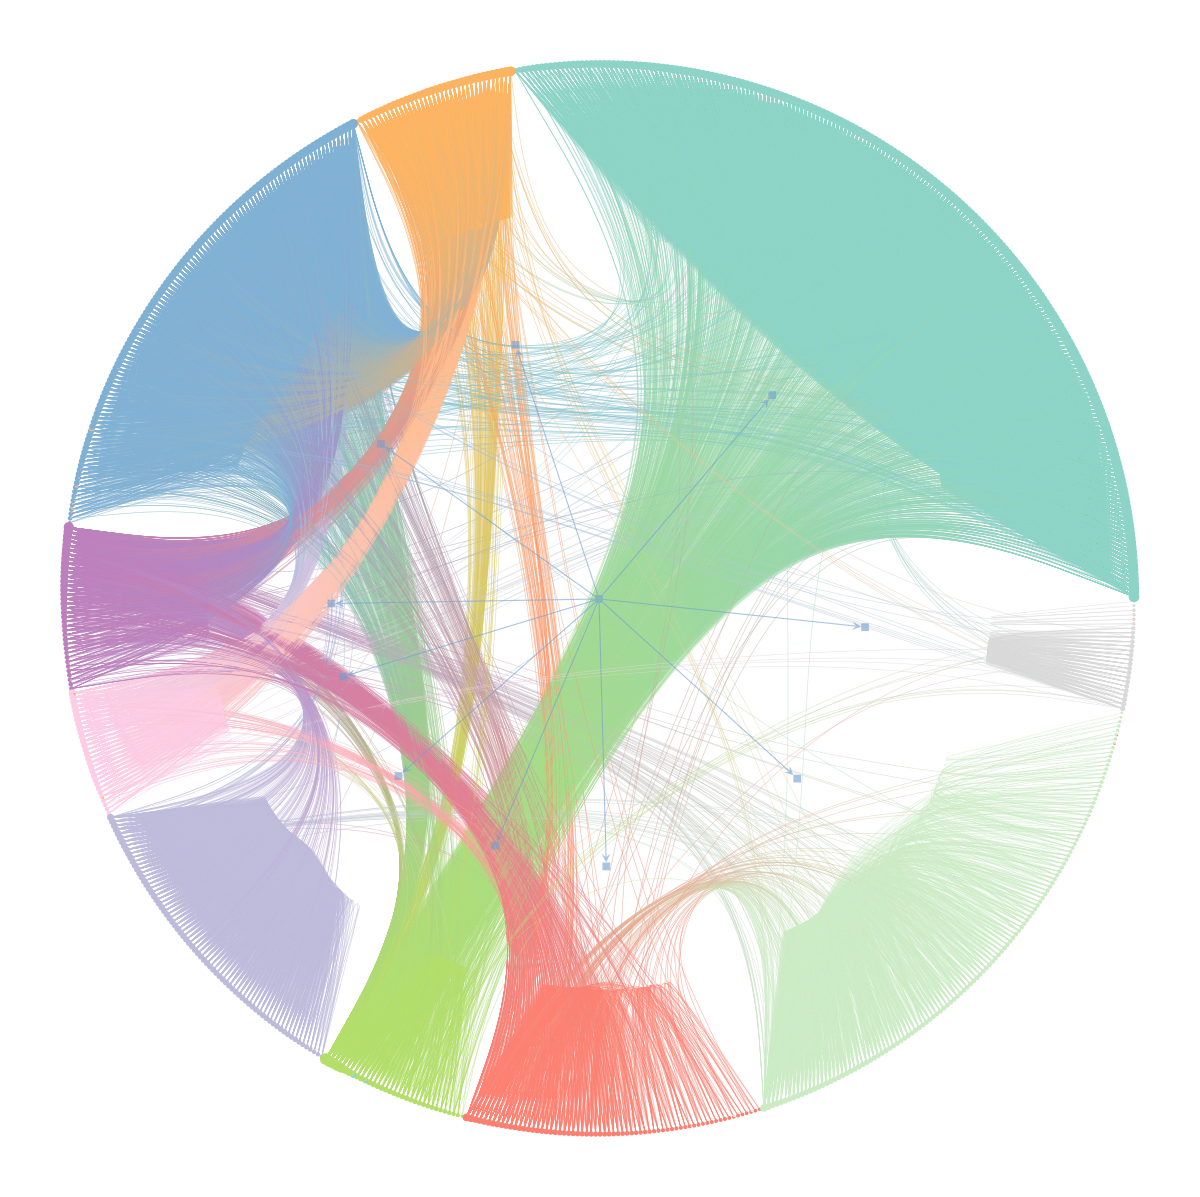
\includegraphics[width=0.28\linewidth]{img/fb-graph.png}
	\caption{Networks laid out and coloured according to inferred block memberships. Left to right: Polbooks, Krebs (2004); Primary School, Stehle et al (2011); Facebook Egonet, Leskovec and Mcauley (2012).}
	\label{fig:graphs-all}
\end{figure}


	\begin{table}[!ht]
	\centering
	\caption{Results averaged over $n=10$ iterations (mean $\pm$ std. dev.).}
	\label{tab:results}
	\resizebox{\textwidth}{!}{%
		\begin{tabular}{c|ccc|c|cc|ccc}
			Dataset  & $B$ & $D$ & $D'$ & $\bar{S}_e$ & $\bar{\mathcal{L}}_0$ & $\bar{\mathcal{L}}_1$ & $c^*$ & $\bar{\mathcal{L}}_0'$ & $\bar{\mathcal{L}}_1'$  \\ \hline
			Polbooks & 3 & 3 & -- & $2.250 \pm 0.000$ & $0.563 \pm 0.042$ & $0.595 \pm 0.089$ & -- & -- & -- \\
			School & 10 & 13 & 10 & $1.894 \pm 0.004$ & $0.787 \pm 0.127$ & $0.885 \pm 0.129$ & $1.198 \pm 0.249$ & $0.793 \pm 0.132$ & $0.853 \pm 0.132$ \\
			FB egonet & 10  & 480 & 10 & $1.626 \pm 0.003$ & $1.326 \pm 0.043$ & $1.538 \pm 0.069$ & $0.94 \pm 0.019$ & $1.580 \pm 0.150$ & $1.605 \pm 0.106$
		\end{tabular}
	}
\end{table}

\begin{figure}[!ht]
	\centering
	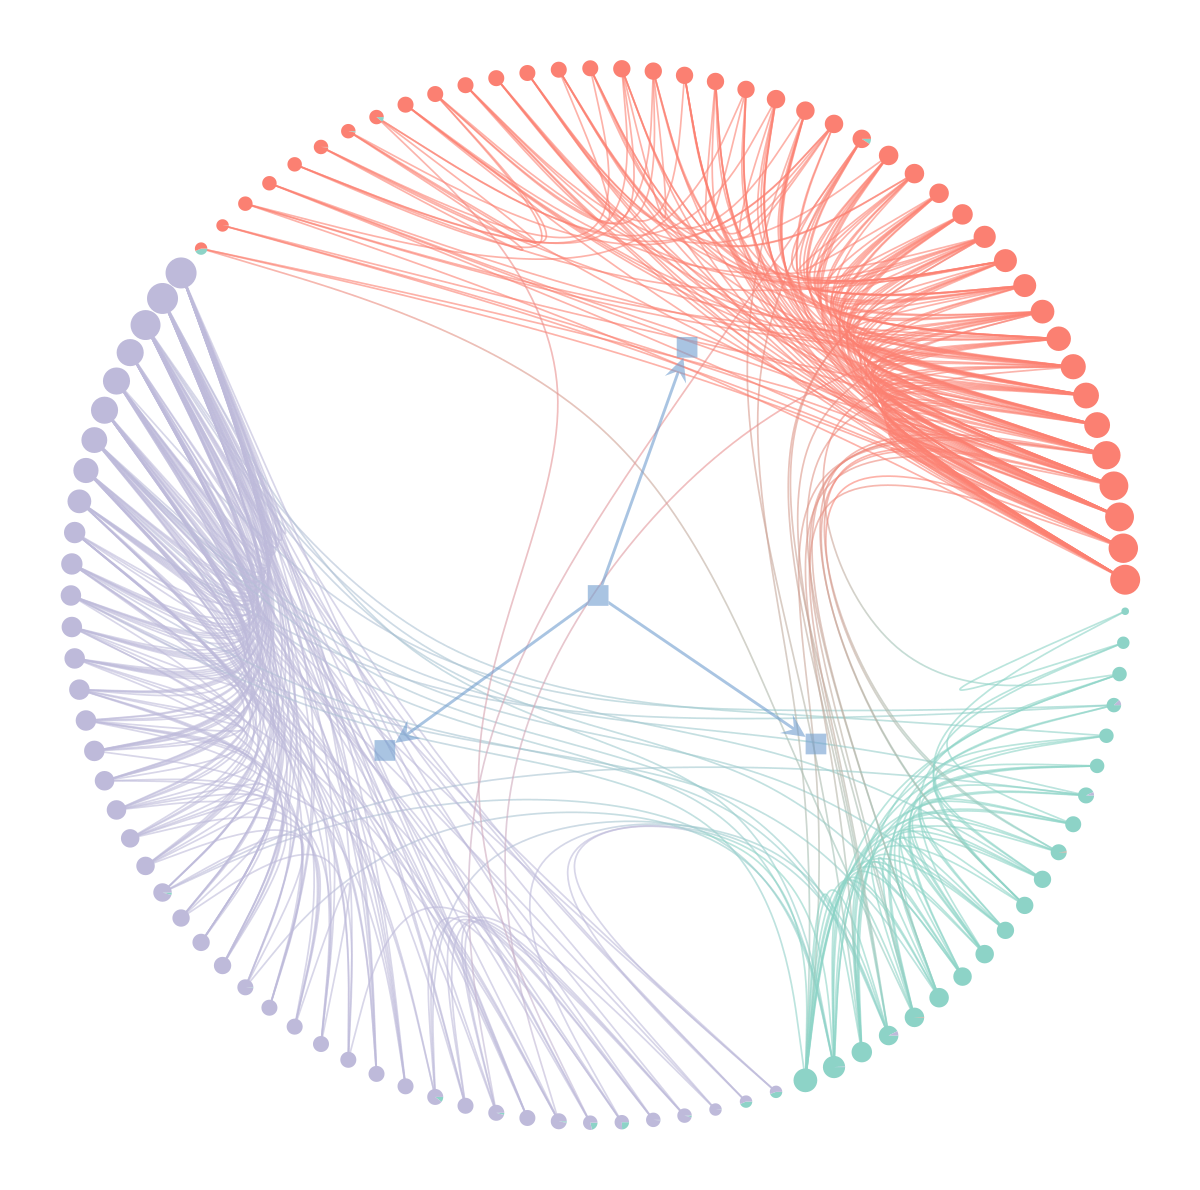
\includegraphics[width=0.28\linewidth]{img/polbooks-graph.png}
	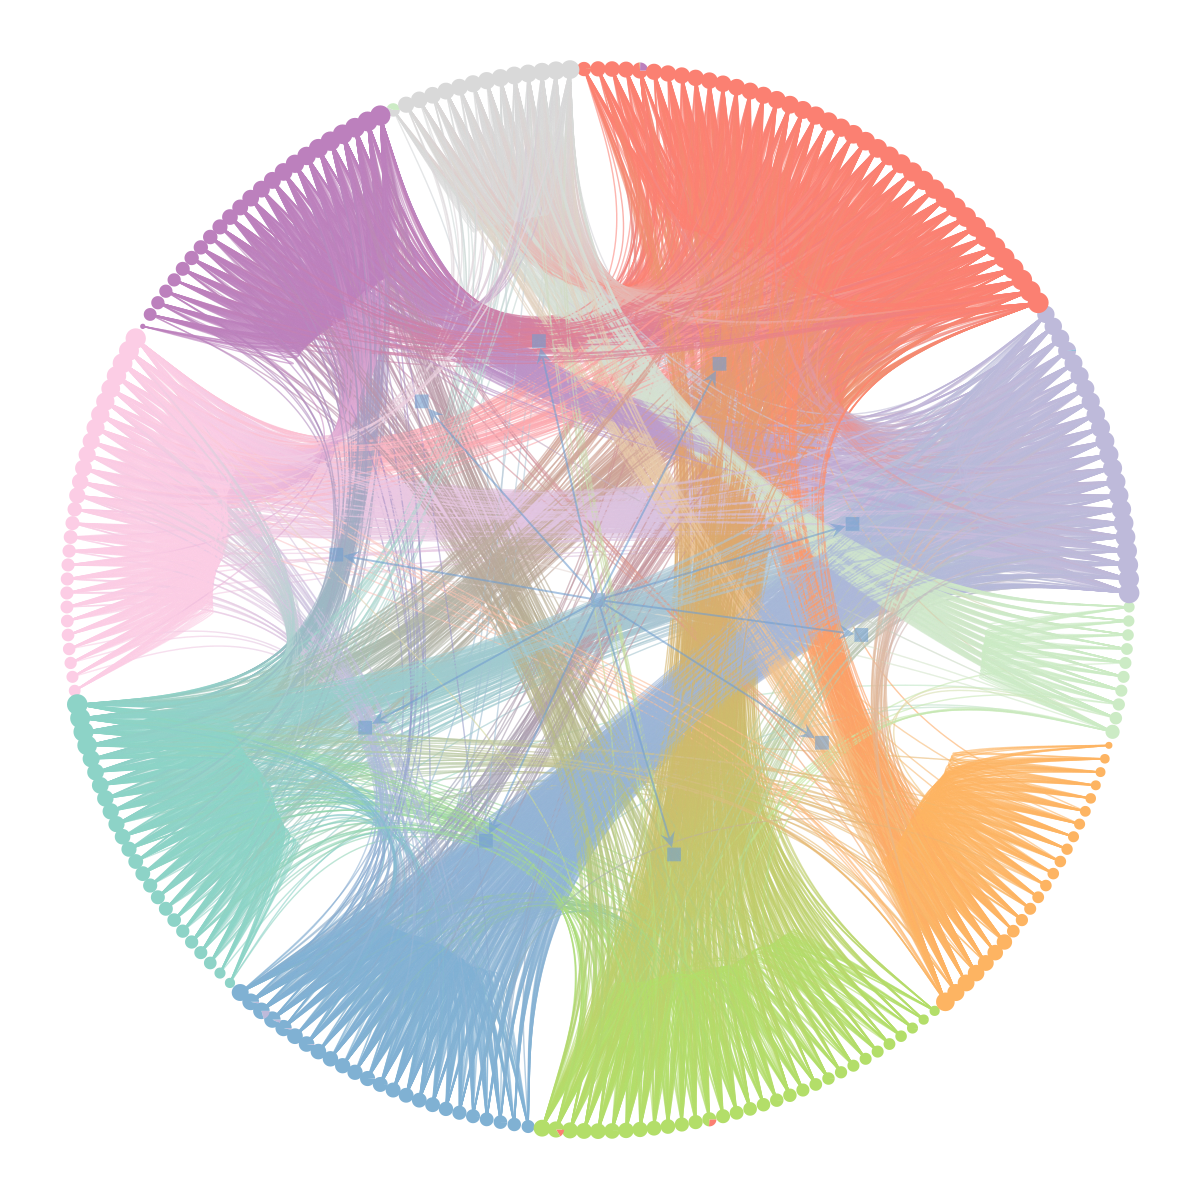
\includegraphics[width=0.28\linewidth]{img/school-graph.png}
	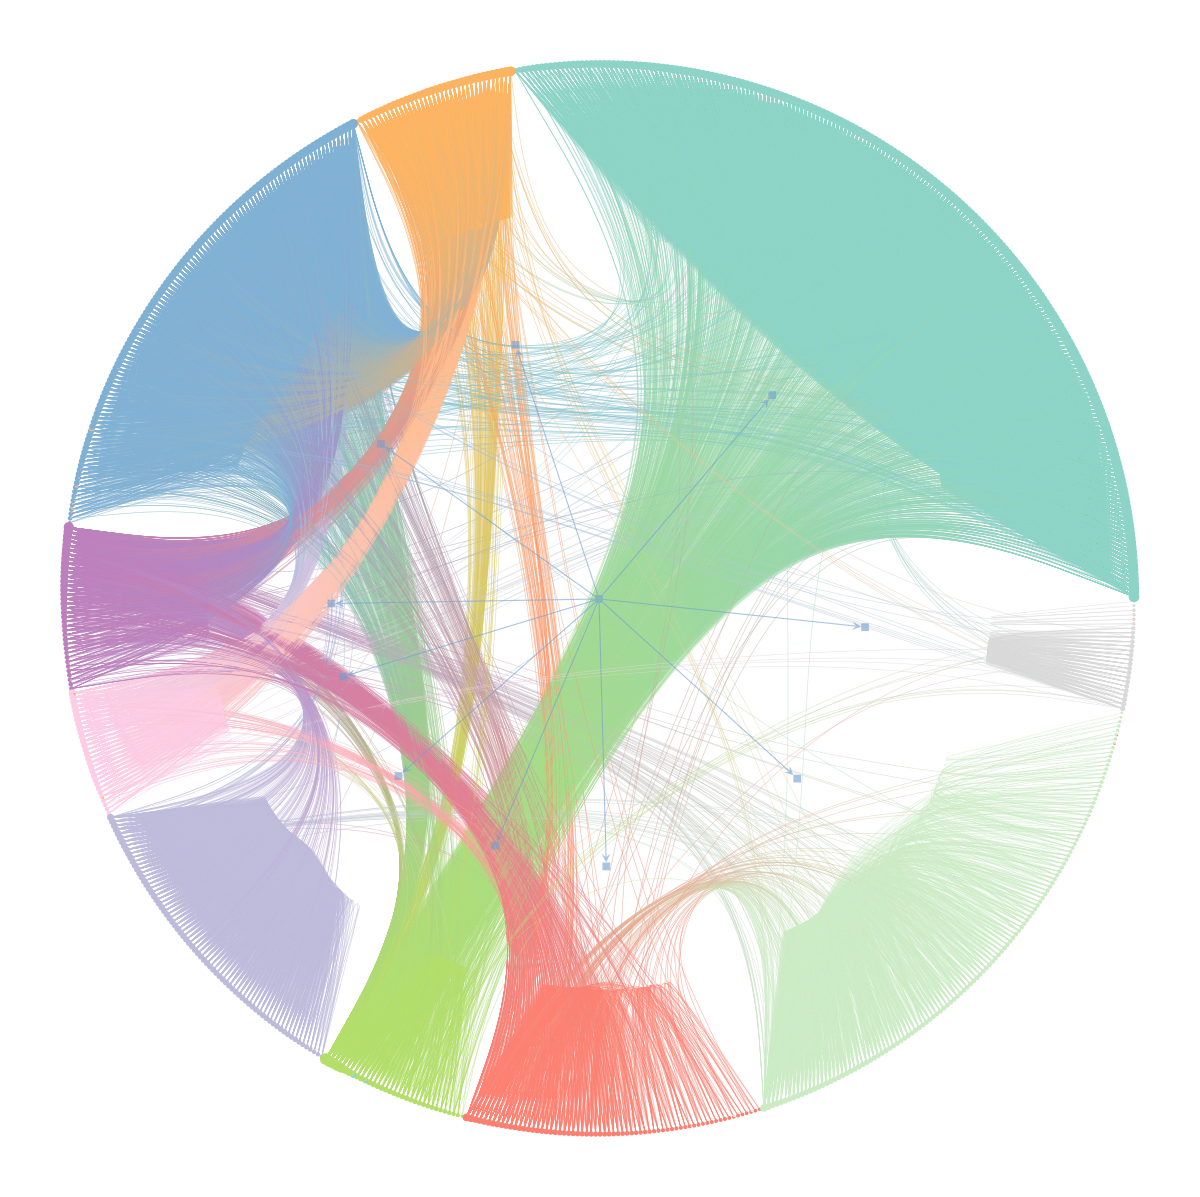
\includegraphics[width=0.28\linewidth]{img/fb-graph.png}
	\caption{Networks laid out and coloured according to inferred block memberships. Left to right: Polbooks, Krebs (2004); Primary School, Stehle et al (2011); Facebook Egonet, Leskovec and Mcauley (2012).}
	\label{fig:graphs-all}
\end{figure}

	%\begin{figure}[!ht]
	\centering
	\begin{subfigure}{0.32\linewidth}
			\centering
			\imagebox{0.9\linewidth}{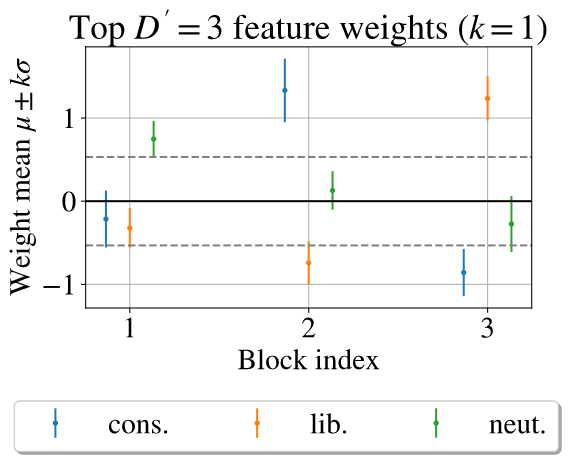
\includegraphics[width=\linewidth]{polbooks-null-1}}
			\caption{Political books}
			\label{fig:polbooks-null}
		\end{subfigure}
	\begin{subfigure}{0.32\linewidth}
			\centering
			\imagebox{0.9\linewidth}{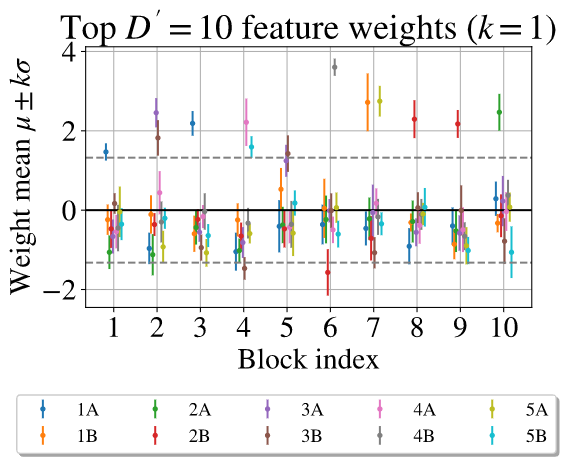
\includegraphics[width=\linewidth]{school-null-1}}
			\caption{Primary school}
			\label{fig:school-null}
		\end{subfigure}
	\begin{subfigure}{0.32\linewidth}
			\centering
			\imagebox{0.9\linewidth}{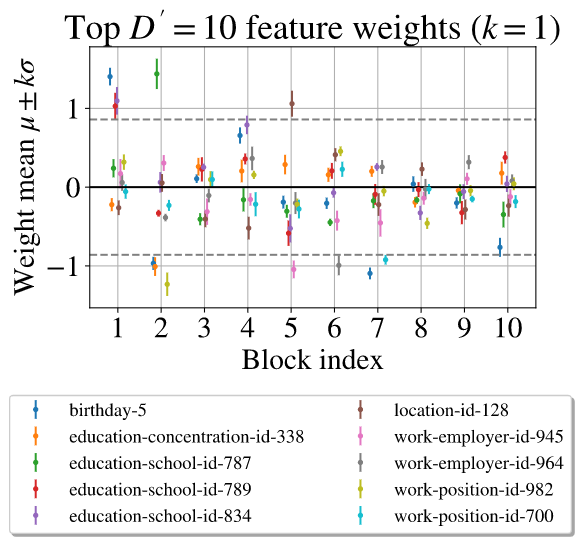
\includegraphics[width=\linewidth]{fb-null-1}}
			\caption{Facebook egonet}
			\label{fig:fb-null}
		\end{subfigure}
	\caption{Top $D'$ $\theta$-samples for each dataset. Coarse steps on x-axis give block index and the fine steps denote give index. Dotted line is $\pm c^*$.}
\end{figure}
%
\begin{figure}[!ht]
	\centering
	\begin{subfigure}{0.32\linewidth}
			\centering
			\imagebox{0.8\linewidth}{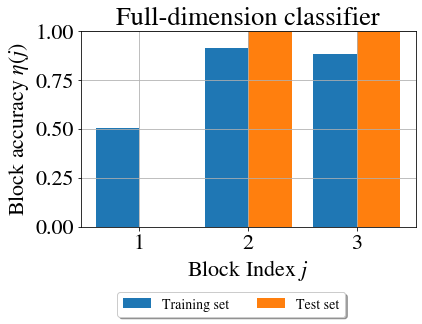
\includegraphics[width=\linewidth]{polbooks-accuracy-2}}
			\caption{Political books}
			\label{fig:polbooks-accuracy}
		\end{subfigure}
	\begin{subfigure}{0.32\linewidth}
			\centering
			\imagebox{0.8\linewidth}{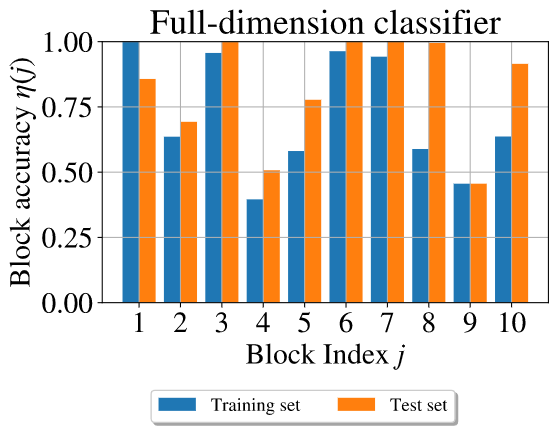
\includegraphics[width=\linewidth]{school-accuracy-1}}
			\caption{Primary school}
			\label{fig:school-accuracy}
		\end{subfigure}
	\begin{subfigure}{0.32\linewidth}
			\centering
			\imagebox{0.8\linewidth}{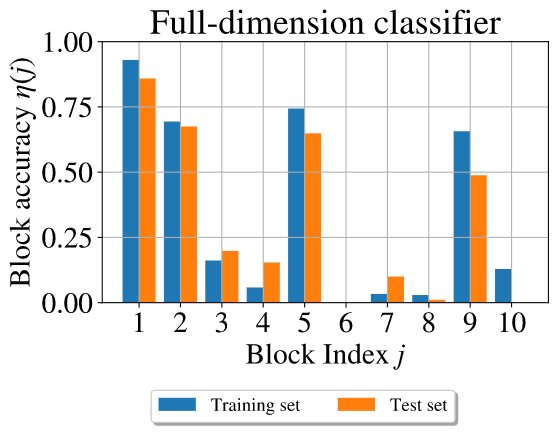
\includegraphics[width=\linewidth]{fb-accuracy-1}}
			\caption{Facebook egonet}
			\label{fig:fb-accuracy}
		\end{subfigure}
	\caption{Per-block accuracy $\eta(j)$ for each dataset.}
\end{figure}
	%Table~\ref{tab:results} summarises the results for each experiment. 
We see that the dimensionality reduction procedure 
brings the training and test losses closer together. This implies that 
the features we keep are indeed correlated with the underlying graphical 
partition and that the approach generalises correctly. The test loss variance is higher than the training loss variance as the test set is smaller and so more susceptible to variability in its construction.
%
The average description length per entity,
$\bar{S}_e$, of the graph, 
has very small variance, suggesting that
the detected communities can be found reliably (to within an arbitrary 
relabelling of blocks).

\paragraph{\textbf{Political books.}}

We choose to partition the network into $B=3$ communities as we only have this many distinct values for political affiliation.
From Figure~\ref{fig:polbooks-null} we see that all 3 blocks have a distinct political affiliation as their largest positive component.  
Furthermore, the training and test losses from Table~\ref{tab:results}  
are very similar and both are low in magnitude. This is strong evidence 
that political affiliation is a very appropriate explanatory 
variable for the overall network structure.
%
However, from Figure~\ref{fig:polbooks-accuracy} we see that block 1 has low accuracy. 
This suggests that detected block 1 is not solely composed of ``neutral" books but also 
contains some ``liberal" and ``conservative" authors. Examining 
Figure~\ref{fig:polbooks-graph}, we see the majority of paths between blocks 2 and 3 go through block 1.
Block 1 is in effect a bridge between the ``conservative'' and ``liberal'' blocks so it is unsurprising that some of these leak into block 1.

\paragraph{\textbf{Primary school.}}

We choose the number of communities $B=10$, in line with the total number of 
school classes. Only the pupils' class memberships (1A-5B) survive
the dimensionality-reduction process (Figure~\ref{fig:school-null});
gender and teacher/student status have been discarded,
meaning these are poor predictors of overall macro-structure.
%
The vast majority of blocks are composed of a single class. 
However, some blocks have two comparably strong classes as their predictors (e.g. blocks 2 and 5). 
Conversely, some classes are found to extend over two 
detected blocks (class 2B spans blocks 8 and 9) but we do 
not have a feature which explains the division.
%
Figure~\ref{fig:school-accuracy} shows excellent accuracy for the majority of blocks. In fact the only blocks with low accuracy are those that have a school-class span two blocks such that we cannot reliably distinguish between the two. This is more pronounced when we apply hard classification rather than the soft cross-entropy loss. Perhaps there are unobserved features which explain this divide.

\paragraph{\textbf{Facebook egonet.}}

The retained features 
(Figure~\ref{fig:fb-null}) are those that best explain the high-level 
community structure. The majority of these are education related. 
Nevertheless, for $D'=10$ we only have good explanations for some of the detected blocks; several blocks in 
Figure~\ref{fig:fb-null} do not have high-magnitude components. This is further emphasised by the disparate accuracies in Figure~\ref{fig:fb-accuracy}.
%
For a high-dimensional feature-space, it is likely that a particular
feature may uniquely identify a small set of vertices; if these are all in the same block, then the classifier may overfit despite the penalty imposed by the prior. Indeed, we see in
Figure~\ref{fig:fb-null} that the feature birthday-5 has a very high weight as it relates to block 1 – but it is unlikely that birthdays determine graphical structure.
	
	%\section{Extensions}

The current FFBM formulation can only explain macro-structure and not structure within each detected block. Future work will benefit from extending the FFBM to be hierarchical in nature. Indeed, the SBM has already been extended to a hierarchical form, often called the nested SBM \cite{SBM-hierarchical}.

The necessary modification of the feature-to-block generator is also rather natural. Given the nested SBM, we would have a hierarchy of generators, each generating a block membership at a particular level of the hierarchy. To avoid exponential growth in the number of model parameters, we could apply some form of dimensionality reduction as we descend the layers so that each generator is only given relevant features as input.
	\section{Conclusion}
\label{sec:conclusion}

The feature-first block model
(FFBM) is introduced, as a 
new generative model for labelled 
networks with communities.
An efficient MCMC algorithm  
is developed for sampling 
from the posterior distribution of
the relevant parameters in the FFBM;
the main idea is to divide up the graph into 
its most natural partition under the associated
parameter values, and then to determine whether 
the vertex features can accurately explain the partition. 
Through applications on empirical
network data, this approach 
is demonstrated to be effective at extracting and describing 
the most natural communities in a labelled network. 
Nevertheless, it
can only currently explain the structure at the macroscopic
scale. Future work will benefit from extending 
the FFBM to a further hierarchical model,
so that
the structure of the network 
can be explained at all scales of interest.



	
	% References should be placed in the text in author (year) form.
% The list of references should be placed below IN ALPHABETICAL ORDER.
% (Please follow the format of the examples very tightly).

\references
\begin{description}

%	\item[Abbe, E.] (2016) Graph compression: The effect of clusters.
%	In: {\it 54th Annual Allerton Conference on Communication, Control, and Computing.}.
	
%	\item[Airoldi, E.M., Blei, D., Fienberg, S., Xing, E.] (2009).
%	Mixed membership stochastic blockmodels. 
%	In: {\it Advances in Neural Information Processing Systems} vol. 21.

%	\item[Gaucher, S., Klopp, O., Robin, G.] (2021).
%	Outliers detection in networks with missing links.
%	Computational Statistics \& Data Analysis 164.
	
	\item[Krebs, V.] (2004) . The political books network,
	http://www.orgnet.com/.

	\item[Leskovec, J., Mcauley, J.] (2012).
	Learning to discover social circles in ego networks.
	{\it Advances in Neural Information Processing Systems} vol. 25

	\item[Nowicki, K., Snijders, T.A.B.] (2001).
	Estimation and prediction for stochastic blockstructures. 
	Journal of the American Statistical Association 96(455), 1077–-1087.

%	\item[Peixoto, T.P.] (2013).
%	The graph-tool Python library. figshare (2014), figshare. com/articles/graph\_tool/1164194
	
%	\item[Peixoto, T.P.] (2014).
%	Efficient Monte Carlo and greedy heuristic for the inference of stochastic block models.
%	Physical Review E 89(1).

	\item[Peixoto, T.P.] (2017).
	Nonparametric Bayesian inference of the microcanonical
	stochastic block model. Physical Review E 95(1).

%	\item[Roberts, G.O., Tweedie, R.L.] (1996).
%	Exponential convergence of Langevin distributions and their discrete approximations.
%	Bernoulli 2(4), 341–-363.

	\item[Stehle, J. et al] (2011).
	High resolution measurements of face-to-face contact patterns in a primary school.
	PLoS ONE 6(8), 1–-13.

%	\item[Zhu, J., Song, J., Chen, B.] (2016).
%	Max-margin nonparametric latent feature models for link prediction.
%	arXiv preprint cs.LG:1602.07428.
\end{description}
	
\end{document}
